\chapter{Urban Source Identification Results and Discussion}

% Compare how well we identify shielded/unshielded isotopes when training set has shielding, doesn't have shielding. 

% Compare how well we identify isotopes over different distances if training set has one vs many distances

% Compare how well we identify isotopes with different calibration sampling granularity 

% https://e-reports-ext.llnl.gov/pdf/312592.pdf holy shit they show common false positive isotopes and we see a lot of overlap



\section{Problem Description and Training Dataset Overview}

This chapter applies machine learning algorithms to solve the problem of identifying a radioactive source in an urban environment where a source may be present. This scenario is applicable when performing source interdiction searching cargo containers, vehicles at boarder crossings, or security at high profile events. Urban environments present unique challenges to gamma-ray spectroscopy. Background radiation can change over city blocks due to different concentrations of uranium and thorium in building materials. Sources may be purposely shielded by unknown amounts of material to obscure their gamma-ray signal.





\section{Data Augmentation Implementation}

Because simulating a dataset with sufficient combinations of available data augmentation - seen in Tables \ref{table:all_fixed_simulation_parameters} and \ref{table:all_variable_simulation_parameters} - online data augmentation techniques are employed. Online data augmentation has the benefit of implicitly regularizing the models.

Steps in the data augmentation process are:
\begin{enumerate}
  \item Randomly choose a background template with the same FWHM as the source template
  \item Rebin source and background template with a random calibration
  \item Apply the LLD to both templates
  \item Normalize both templates by the sum of their respective counts 
  \item Scale both signals by their respective total counts
  \begin{itemize}
     \item Counts defined by randomly chosen background counts per second, integration time, and signal to background ratio
   \end{itemize}
  \item Add both signals 
  \item Poisson sample the resulting signal
\end{enumerate}


\section{Learning Curve Comparison for Fixed-size Datasets and Online Data Augmentation Datasets}

In this section we use learning curves to quantify how well the online data augmentation improved testing error. Learning curves are [definition, explanation]. Learning curves are used to determine a few things. We will use them to do [the following].

First, They are used as a sanity check, to make sure we are sampling our input space with enough granularity. To know we are sampling well enough, we should be sampling in a region where the curves are flat for both algorithms.

Secondly, Learning curves give us insight into which algorithm works better on the hyperparameter optimization dataset and simplified version of the problem. We're expecting the CNN to outperform the DNN due to theoretical benefits of convolution architectures for our problem. We can also compare this curve to the final learning curves for the final datasets.

For the autoencoders, pretraining was done using a fixed dataset of 10000 samples. Because of the implicit regularization of the undercomplete encoding and the denoising background subtracting process, both networks do not use a additional regularization when training. The initial learning rate of each autoencoder was set to 10$^{-5}$.


\begin{figure}[H]
	\centering
	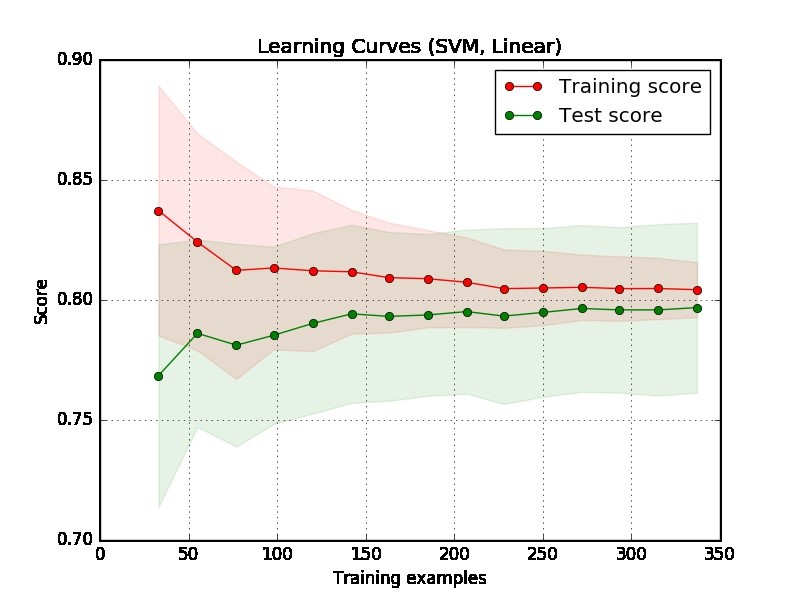
\includegraphics[width=0.8\linewidth]{model_choice_hyperparameter_search_images/learning_curve_dummy}
	\caption{Learning curves from the best DNN with best performance from online data augmentation. Shown: learning curve example.}
	\label{fig:learning_curves}
\end{figure}



\begin{figure}[H]
	\centering
	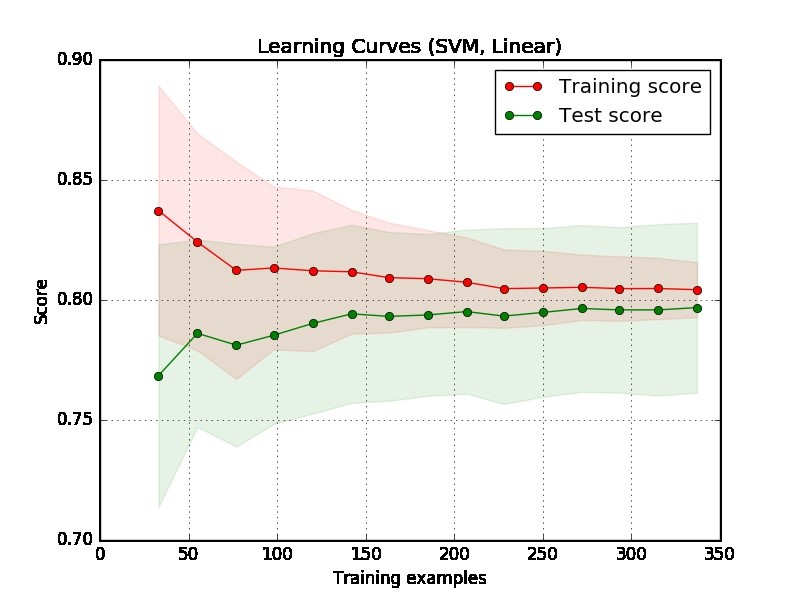
\includegraphics[width=0.8\linewidth]{model_choice_hyperparameter_search_images/learning_curve_dummy}
	\caption{Learning curves from the best CNN with best performance from online data augmentation. Shown: learning curve example.}
	\label{fig:learning_curves}
\end{figure}


\section{Generalization Performance Evaluation}

In this section we analyze the generalization performance of each network and training dataset. To quantify performance on a range of spectra qualities, the F1-scores for each bagged model are shown over integration time and signal to background ratios of 0.1 and 0.5. Default simulation parameters are shown in Table \ref{table:default_sim_params}. Changes to these defaults are indicated for each generalization experiment. For each generalization dataset, ten spectra are generated for each isotope using the indicated simulation parameters.

\begin{table}[H]
\centering
\caption{Default parameters used for all generalization datasets.}
\label{table:default_sim_params}
\begin{tabular}{cc}
% \cline{2-3}
Hyperparameter &  Value \\ \hline
\multicolumn{1}{c}{Source-Detector Distance {[}cm{]}} & 175.0\\ 
\multicolumn{1}{c}{Source-Detector Height {[}cm{]}} & 100.0\\ 
\multicolumn{1}{c}{FWHM 662 keV {[}s{]}} & 7.0\\ 
\multicolumn{1}{c}{\begin{tabular}[c]{@{}c@{}}Shielding\\ (Percent 200 keV Attenuated)\end{tabular}} & 0\% \\ 
% \multicolumn{1}{c}{Integration Time {[}s{]}} & 60 - 600 \\ 
\multicolumn{1}{c}{Calibration - Offset (channels)} & 0 \\ 
\multicolumn{1}{c}{Calibration - Gain} & 1.0 \\ 
% \multicolumn{1}{c}{Signal to Background Ratio} & 0.5 - 2.0 \\ 
\multicolumn{1}{c}{Background Counts Per Second} & 200 \\ 
\end{tabular}
\end{table}


% \begin{figure}[H]
%      \centering
%      \begin{subfigure}[b]{0.49\textwidth}
%          \centering
%          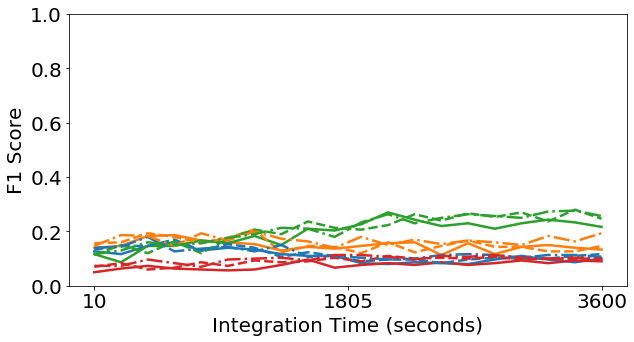
\includegraphics[width=\textwidth]{images/generalization-height-easy-01.png}
%          \caption{}
%          \label{fig:generalization-height-easy-01}
%      \end{subfigure}
%      \hfill
%      \begin{subfigure}[b]{0.49\textwidth}
%          \centering
%          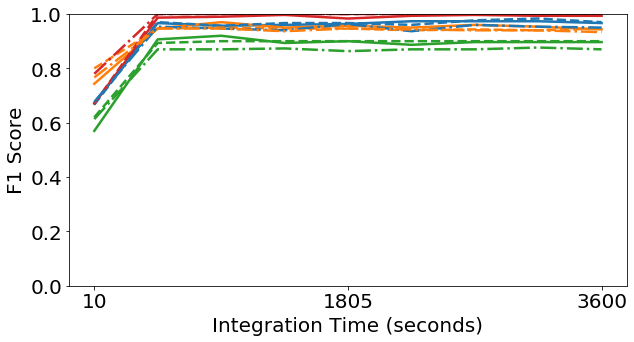
\includegraphics[width=\textwidth]{images/generalization-height-easy-05.png}
%          \caption{}
%          \label{fig:generalization-height-easy-05}
%      \end{subfigure}

%         \caption{Examples of spectra simulated with different signal-to-background ratios,}
%         \label{fig:generalization_signalbackground_examples}
% \end{figure}


% When the error between models differs significantly or is particularly large, confusion matrices are included to show what isotopes are problematic.

\newcommand{\blackline}{\raisebox{2pt}{\tikz{\draw[-,black!40!black,solid,line width = 1.1pt](0,0) -- (6mm,0);}}}

\newcommand{\blackdotline}{\raisebox{2pt}{\tikz{\draw[-,black!40!black,dashed,line width = 1.1pt](0,0) -- (6mm,0);}}}

\newcommand{\blackdashdotline}{\raisebox{2pt}{\tikz{\draw[-,black!40!black,dash dot,line width = 1.1pt](0,0) -- (6mm,0);}}}


\subsection{Generalization Performance on Source-Detector Height}

In this section we analyze the generalization performance of each network on changes in source-detector height from ground. This analysis tests if each model is sensitive to changes in the Compton continuum due to environmental scattering associated with the source-detector height. An example of these changes can be seen in Figure \ref{fig:sim_spectra_height_comparison}.

As seen in Figure \ref{fig:generalization_height_fixeddataset}, the performance of each network was not significantly changed with changes to source-detector height. This shows that the small changes in the Compton continuum caused by varying the source-detector height. The CNN performed the best in all cases except when trained on the simple dataset and identifying spectra at a signal-to-noise ratio below the range used in the simple dataset. This Figure also shows that the simple dataset generalized to changes in source-detector height. The DAE did not perform well in the complete dataset, indicating that either the pretraining produced a poor encoding that was difficult to fine-tune through further training.

Models trained on the simple dataset did not generalize well to low signal-to-background data, shown in \ref{fig:generalization-height-easy-01}. The DNN significantly outperformed the other models in this dataset. This is consistent with the thought that the DNN is using a ROI approach to identification and the CNN is using more abstract features. Because the scale of the abstract features (like those associated with the Compton continuum) are very different at a signal-to-background ratio of 0.1 compared to 0.5, the features used by the CNN trained on the simple dataset would be very different from those required by the parameters used by the complete dataset.


\begin{figure}[H]
     \centering
     \begin{subfigure}[b]{0.49\textwidth}
         \centering
         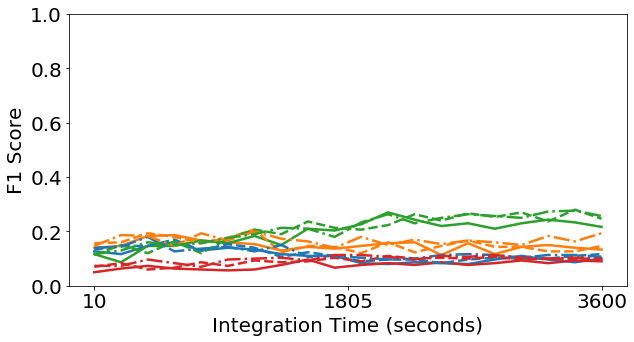
\includegraphics[width=\textwidth]{images/generalization-height-easy-01.png}
         \caption{}
         \label{fig:generalization-height-easy-01}
     \end{subfigure}
     \hfill
     \begin{subfigure}[b]{0.49\textwidth}
         \centering
         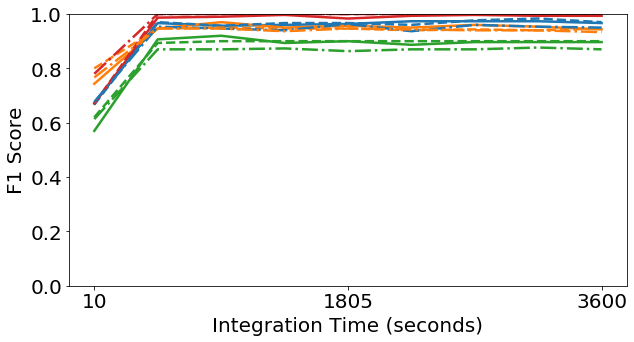
\includegraphics[width=\textwidth]{images/generalization-height-easy-05.png}
         \caption{}
         \label{fig:generalization-height-easy-05}
     \end{subfigure}

     \begin{subfigure}[b]{0.49\textwidth}
         \centering
         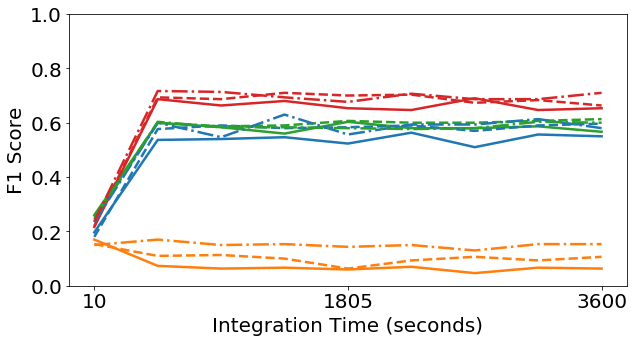
\includegraphics[width=\textwidth]{images/generalization-height-full-01.png}
         \caption{}
         \label{fig:generalization-height-full-01}
     \end{subfigure}
     \hfill
     \begin{subfigure}[b]{0.49\textwidth}
         \centering
         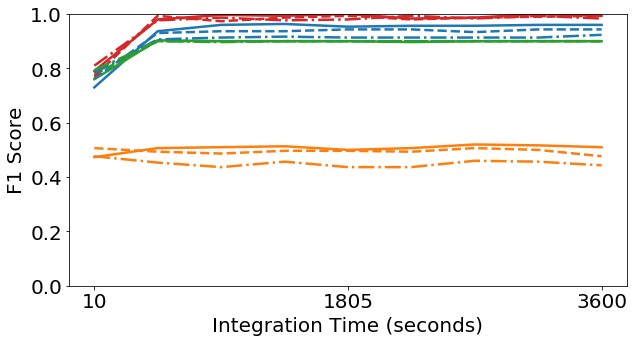
\includegraphics[width=\textwidth]{images/generalization-height-full-05.png}
         \caption{}
         \label{fig:generalization-height-full-05}
     \end{subfigure}
    % \begin{tabular}{r@{: }l r@{: }l}
    \begin{tabular}{r@{: }l r@{: }l r@{: }l r@{: }l}
    DNN & Green & CNN & Red & DAE & Yellow & CAE & Blue\\
    \end{tabular}
    \begin{tabular}{r@{: }l r@{: }l r@{: }l}
    50 cm & \blackline & 100 cm & \blackdotline & 150 cm & \blackdashdotline
    \end{tabular}
        \caption{Height-off-ground generalization performance of the DNN, CNN with and without autoencoder pretraining. The F1 score is averaged over five networks trained with 10000 total dataset examples. Figures in the top and bottom row are trained using the simple and complete dataset and Figures in the first and second column are use spectra with signal-to-noise ratios of 0.1 and 0.5, respectively.}
        \label{fig:generalization_height_fixeddataset}
\end{figure}

The performance using online data augmentation are shown in Figure \ref{fig:generalization_height_augdataset}. General trends in performance, such as the CNN performing very well and the DAE trained on the complete dataset performing poorly, are similar between models trained with a fixed-dataset and models trained with online data augmentation. Differences include reduced performance for most models.

\begin{figure}[H]
     \centering
     \begin{subfigure}[b]{0.49\textwidth}
         \centering
         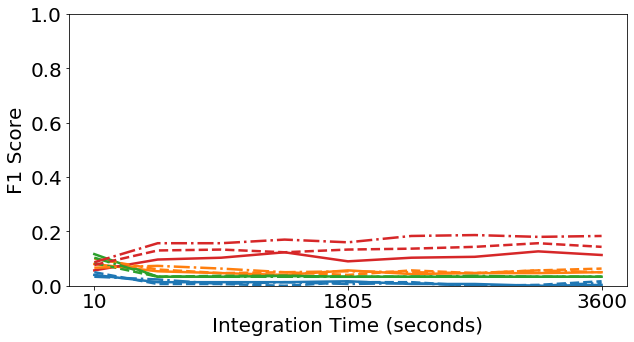
\includegraphics[width=\textwidth]{images/generalization-height-aug-easy-01.png}
         \caption{}
         \label{fig:generalization-height-aug-easy-01}
     \end{subfigure}
     \hfill
     \begin{subfigure}[b]{0.49\textwidth}
         \centering
         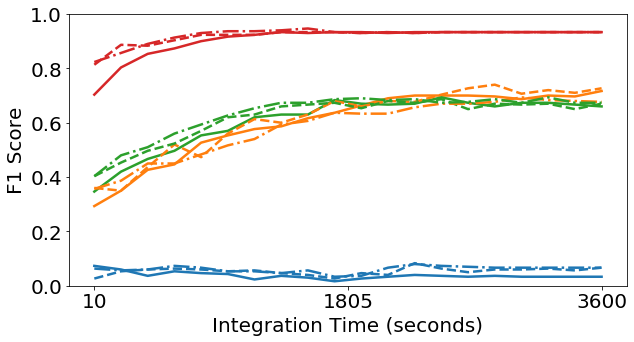
\includegraphics[width=\textwidth]{images/generalization-height-aug-easy-05.png}
         \caption{}
         \label{fig:generalization-height-aug-easy-05}
     \end{subfigure}

     \begin{subfigure}[b]{0.49\textwidth}
         \centering
         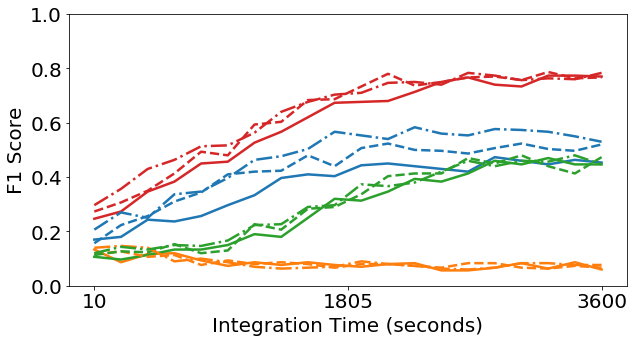
\includegraphics[width=\textwidth]{images/generalization-height-aug-full-01.png}
         \caption{}
         \label{fig:generalization-height-aug-full-01}
     \end{subfigure}
     \hfill
     \begin{subfigure}[b]{0.49\textwidth}
         \centering
         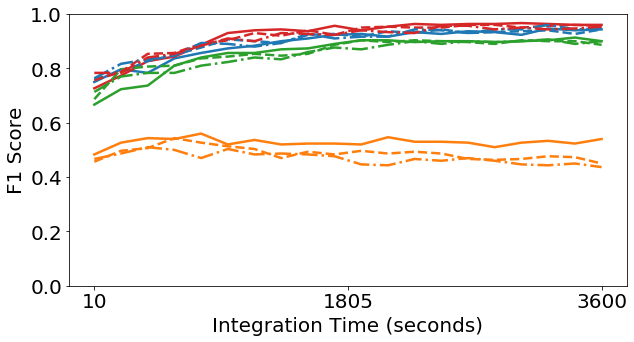
\includegraphics[width=\textwidth]{images/generalization-height-aug-full-05.png}
         \caption{}
         \label{fig:generalization-height-aug-full-05}
     \end{subfigure}
    \begin{tabular}{r@{: }l r@{: }l r@{: }l r@{: }l}
    DNN & Green & CNN & Red & DAE & Yellow & CAE & Blue\\
    \end{tabular}
    \begin{tabular}{r@{: }l r@{: }l r@{: }l}
    50 cm & \blackline & 100 cm & \blackdotline & 150 cm & \blackdashdotline
    \end{tabular}
        \caption{Height-off-ground generalization performance of the DNN, CNN with and without autoencoder pretraining. The F1 score is averaged over five networks trained with data augmentation, Figures in the top and bottom row are trained using the simple and complete dataset and Figures in the first and second column are use spectra with signal-to-noise ratios of 0.1 and 0.5, respectively.}
        \label{fig:generalization_height_augdataset}
\end{figure}

\subsection{Generalization Performance on Source-Detector Standoff Distance}

In this section we analyze the generalization performance of each network on changes in source-detector standoff distance. This analysis tests if each model is sensitive to larger changes in the Compton continuum compared to those associated with the source-detector height. An example of these changes can be seen in Figure \ref{fig:sim_spectra_distance_comparison}.

As seen in Figure \ref{fig:generalization_dist_fixeddataset}, general trends seen in the source-detector height generalization, such as the superior performance of the CNN and the poor DAE encoding, are observed in source-detector distance generalization. There are a number of differences in performance, including more significant changes in performance when compared to changes in standoff distance. This change was especially noticeable for the shorter standoff distance of 50 cm. At this distance, the peak-to-total ratio increases significantly, which emphasizes the peak information while reducing the Compton continuum. Interestingly, at low signal-to-background ratios the closer standoff distance improves performance in each network and training dataset while at higher signal-to-background ratios this trend is reversed. Higher peak-to-total ratios make identification easier for algorithms that focus on photopeaks. The reduced performance of each model on high peak-to-total ratio spectra on the higher signal-to-background data shows that the models are acting more similarly to a template matching than a ROI approach. 






\begin{figure}[H]
     \centering
     \begin{subfigure}[b]{0.49\textwidth}
         \centering
         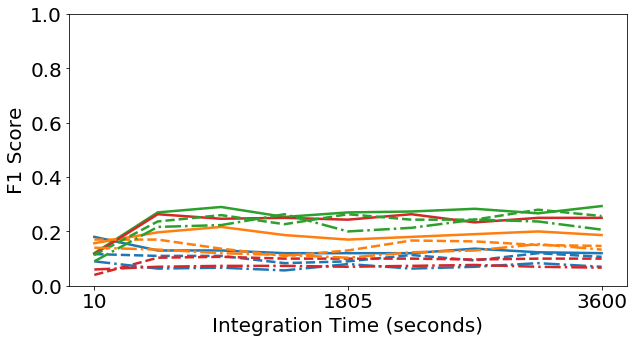
\includegraphics[width=\textwidth]{images/generalization-dist-easy-01.png}
         \caption{}
         \label{fig:generalization-dist-easy-01}
     \end{subfigure}
     \hfill
     \begin{subfigure}[b]{0.49\textwidth}
         \centering
         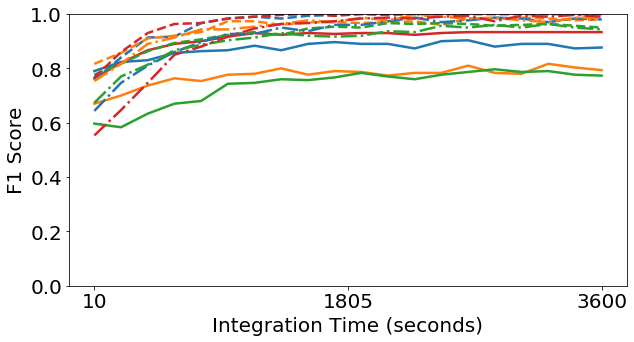
\includegraphics[width=\textwidth]{images/generalization-dist-easy-05.png}
         \caption{}
         \label{fig:generalization-dist-easy-05}
     \end{subfigure}

     \begin{subfigure}[b]{0.49\textwidth}
         \centering
         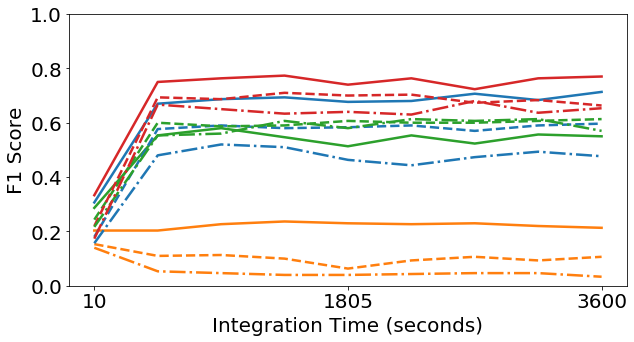
\includegraphics[width=\textwidth]{images/generalization-dist-full-01.png}
         \caption{}
         \label{fig:generalization-dist-full-01}
     \end{subfigure}
     \hfill
     \begin{subfigure}[b]{0.49\textwidth}
         \centering
         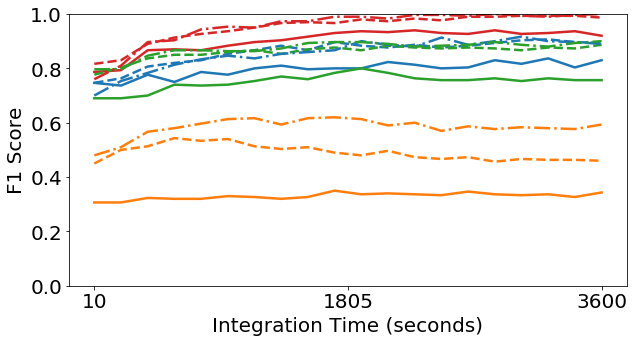
\includegraphics[width=\textwidth]{images/generalization-dist-full-05.png}
         \caption{}
         \label{fig:generalization-dist-full-05}
     \end{subfigure}
    \begin{tabular}{r@{: }l r@{: }l r@{: }l r@{: }l}
    DNN & Green & CNN & Red & DAE & Yellow & CAE & Blue\\
    \end{tabular}
    \begin{tabular}{r@{: }l r@{: }l r@{: }l}
    50 cm & \blackline & 175 cm & \blackdotline & 300 cm & \blackdashdotline
    \end{tabular}
        \caption{Standoff distance generalization performance of the DNN, CNN with and without autoencoder pretraining. F1 score shown in averaged over five networks trained with 10000 total dataset examples, Figures in the top and bottom row are trained using the simple and complete dataset and Figures in the first and second column are use spectra with signal-to-noise ratios of 0.1 and 0.5, respectively.}
        \label{fig:generalization_dist_fixeddataset}
\end{figure}


Training with online data augmentation again reduced performance in all models except the CNN. The CNN's performance improved significantly at a low signal-to-background ratio at a standoff distance of 50 cm, seen in Figure \ref{fig:generalization-dist-aug-easy-01}. This boost in performance tied with the CNN performance not reducing like the other models trained using online data augmentation may show that CNN models can benefit from this aggressive training technique. 


\begin{figure}[H]
     \centering
     \begin{subfigure}[b]{0.49\textwidth}
         \centering
         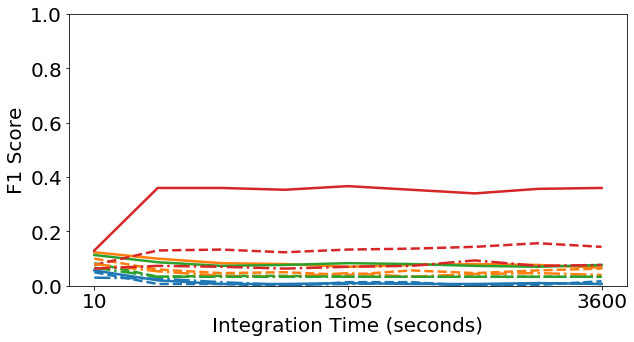
\includegraphics[width=\textwidth]{images/generalization-dist-aug-easy-01.png}
         \caption{}
         \label{fig:generalization-dist-aug-easy-01}
     \end{subfigure}
     \hfill
     \begin{subfigure}[b]{0.49\textwidth}
         \centering
         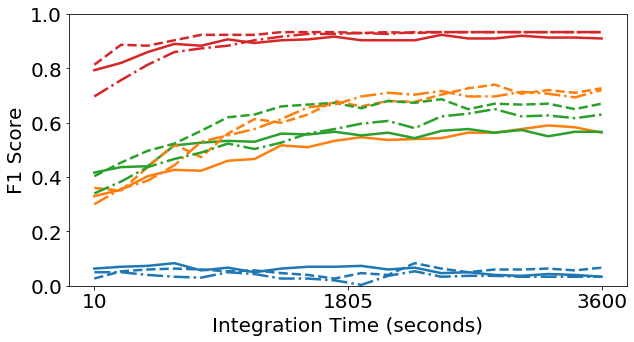
\includegraphics[width=\textwidth]{images/generalization-dist-aug-easy-05.png}
         \caption{}
         \label{fig:generalization-dist-aug-easy-05}
     \end{subfigure}

     \begin{subfigure}[b]{0.49\textwidth}
         \centering
         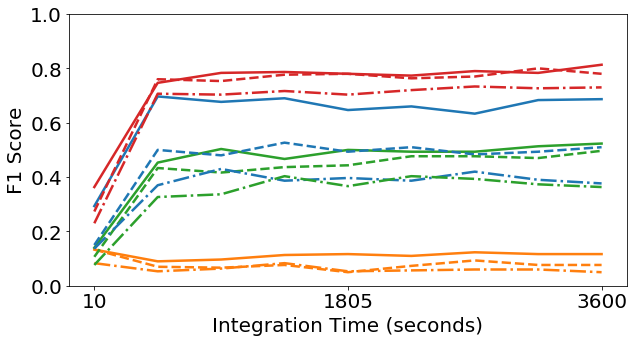
\includegraphics[width=\textwidth]{images/generalization-dist-aug-full-01.png}
         \caption{}
         \label{fig:generalization-dist-aug-full-01}
     \end{subfigure}
     \hfill
     \begin{subfigure}[b]{0.49\textwidth}
         \centering
         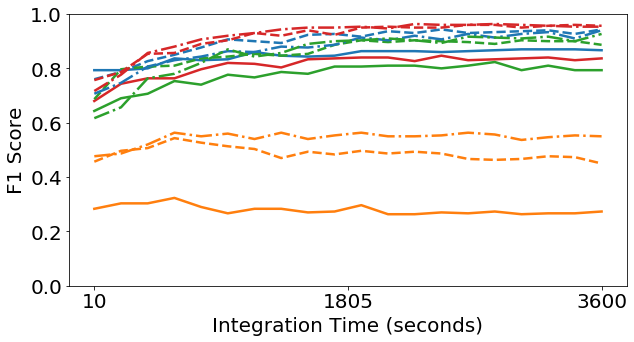
\includegraphics[width=\textwidth]{images/generalization-dist-aug-full-05.png}
         \caption{}
         \label{fig:generalization-dist-aug-full-05}
     \end{subfigure}
    \begin{tabular}{r@{: }l r@{: }l r@{: }l r@{: }l}
    DNN & Green & CNN & Red & DAE & Yellow & CAE & Blue\\
    \end{tabular}
    \begin{tabular}{r@{: }l r@{: }l r@{: }l}
    50 cm & \blackline & 175 cm & \blackdotline & 300 cm & \blackdashdotline
    \end{tabular}
        \caption{Standoff distance generalization performance of the DNN, CNN with and without autoencoder pretraining. F1 score shown in averaged over five networks trained with data augmentation, Figures in the top and bottom row are trained using the simple and complete dataset and Figures in the first and second column are use spectra with signal-to-noise ratios of 0.1 and 0.5, respectively.}
        \label{fig:generalization_dist_augdataset}
\end{figure}



\subsection{Generalization Dependence on Resolution}

In this section we analyze the generalization performance of each network on changes in detector resolution. An example of these changes can be seen in Figure \ref{fig:sim_spectra_FWHM_comparison}.

Changes in resolution do not significantly impact performance of any model. Trends are similar to distance and height generalization.


\begin{figure}[H]
     \centering
     \begin{subfigure}[b]{0.49\textwidth}
         \centering
         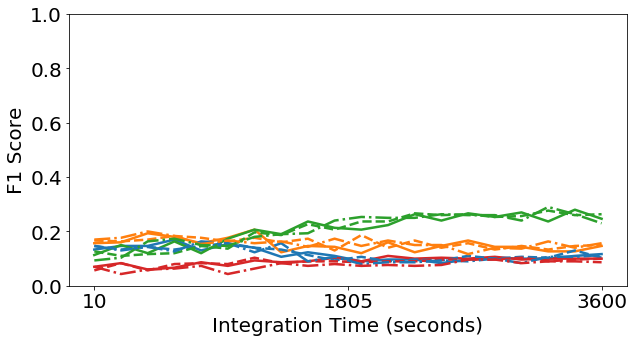
\includegraphics[width=\textwidth]{images/generalization-fwhm-easy-01.png}
         \caption{}
         \label{fig:generalization-fwhm-easy-01}
     \end{subfigure}
     \hfill
     \begin{subfigure}[b]{0.49\textwidth}
         \centering
         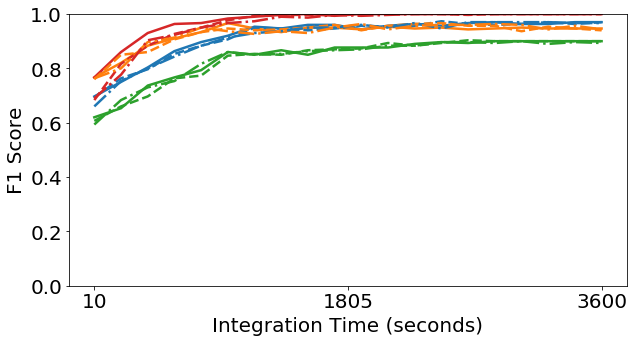
\includegraphics[width=\textwidth]{images/generalization-fwhm-easy-05.png}
         \caption{}
         \label{fig:generalization-fwhm-easy-05}
     \end{subfigure}

     \begin{subfigure}[b]{0.49\textwidth}
         \centering
         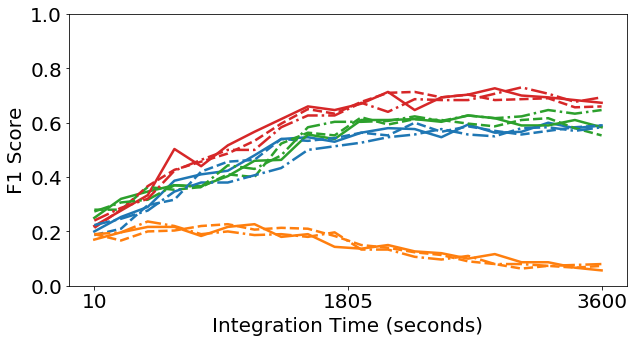
\includegraphics[width=\textwidth]{images/generalization-fwhm-full-01.png}
         \caption{}
         \label{fig:generalization-fwhm-full-01}
     \end{subfigure}
     \hfill
     \begin{subfigure}[b]{0.49\textwidth}
         \centering
         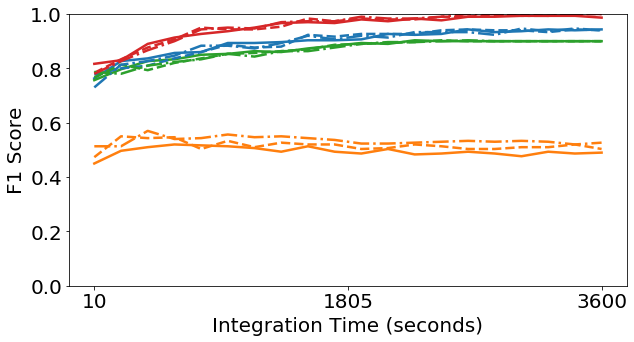
\includegraphics[width=\textwidth]{images/generalization-fwhm-full-05.png}
         \caption{}
         \label{fig:generalization-fwhm-full-05}
     \end{subfigure}
    \begin{tabular}{r@{: }l r@{: }l r@{: }l r@{: }l}
    DNN & Green & CNN & Red & DAE & Yellow & CAE & Blue\\
    \end{tabular}
    \begin{tabular}{r@{: }l r@{: }l r@{: }l}
    7.0 & \blackline & 7.5 & \blackdotline & 8.0 & \blackdashdotline
    \end{tabular}
        \caption{Resolution generalization performance of the DNN, CNN with and without autoencoder pretraining. Resolutions in legend are measured at 662 keV. F1 score shown in averaged over five networks trained with data augmentation, Figures in the top and bottom row are trained using the simple and complete dataset and Figures in the first and second column are use spectra with signal-to-noise ratios of 0.1 and 0.5, respectively.}
        \label{fig:generalization_fwhm_fixeddataset}
\end{figure}




\begin{figure}[H]
     \centering
     \begin{subfigure}[b]{0.49\textwidth}
         \centering
         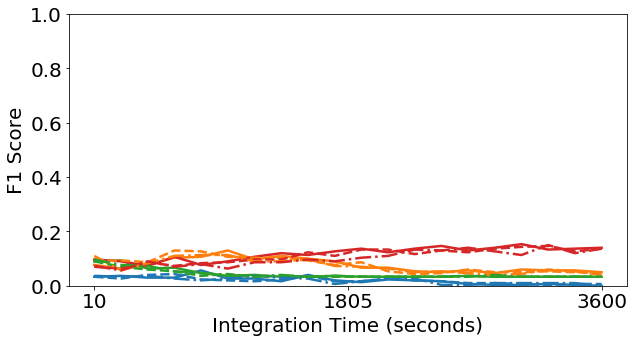
\includegraphics[width=\textwidth]{images/generalization-fwhm-aug-easy-01.png}
         \caption{}
         \label{fig:generalization-fwhm-aug-easy-01}
     \end{subfigure}
     \hfill
     \begin{subfigure}[b]{0.49\textwidth}
         \centering
         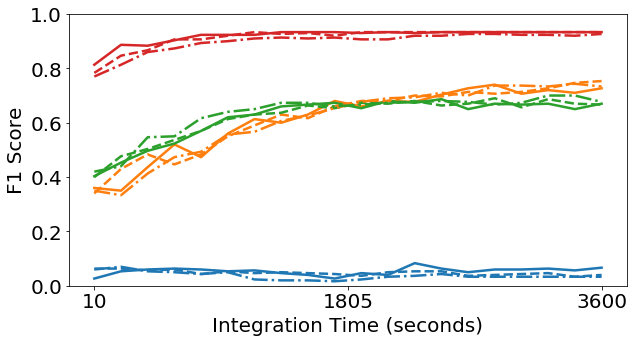
\includegraphics[width=\textwidth]{images/generalization-fwhm-aug-easy-05.png}
         \caption{}
         \label{fig:generalization-fwhm-aug-easy-05}
     \end{subfigure}

     \begin{subfigure}[b]{0.49\textwidth}
         \centering
         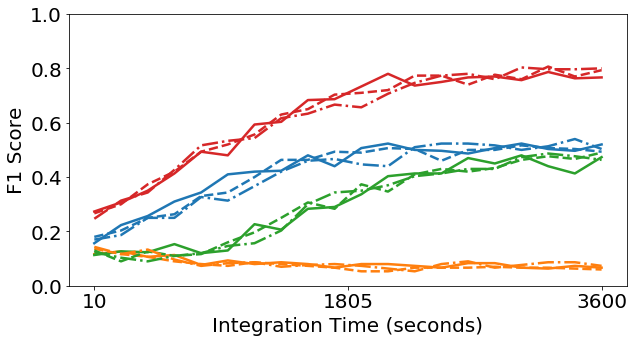
\includegraphics[width=\textwidth]{images/generalization-fwhm-aug-full-01.png}
         \caption{}
         \label{fig:generalization-fwhm-aug-full-01}
     \end{subfigure}
     \hfill
     \begin{subfigure}[b]{0.49\textwidth}
         \centering
         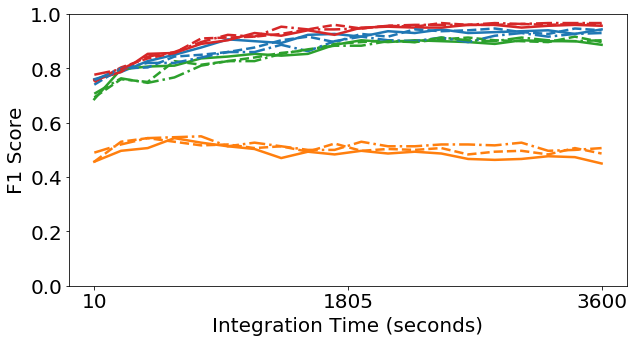
\includegraphics[width=\textwidth]{images/generalization-fwhm-aug-full-05.png}
         \caption{}
         \label{fig:generalization-fwhm-aug-full-05}
     \end{subfigure}
    \begin{tabular}{r@{: }l r@{: }l r@{: }l r@{: }l}
    DNN & Green & CNN & Red & DAE & Yellow & CAE & Blue\\
    \end{tabular}
    \begin{tabular}{r@{: }l r@{: }l r@{: }l}
    7.0 & \blackline & 7.5 & \blackdotline & 8.0 & \blackdashdotline
    \end{tabular}
        \caption{Resolution generalization performance of the DNN, CNN with and without autoencoder pretraining. Resolutions in legend are measured at 662 keV. F1 score shown in averaged over five networks trained with data augmentation, Figures in the top and bottom row are trained using the simple and complete dataset and Figures in the first and second column are use spectra with signal-to-noise ratios of 0.1 and 0.5, respectively.}
        \label{fig:generalization_fwhm_augdataset}
\end{figure}


\subsection{Generalization Dependence on Shielding.}

In this section we analyze the generalization performance of each network on changes in shielding.



\begin{figure}[H]
     \centering
     \begin{subfigure}[b]{0.49\textwidth}
         \centering
         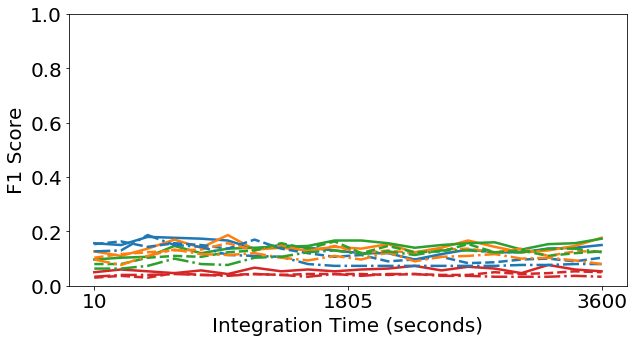
\includegraphics[width=\textwidth]{images/generalization-shielding-easy-01.png}
         \caption{}
         \label{fig:generalization-shielding-easy-01}
     \end{subfigure}
     \hfill
     \begin{subfigure}[b]{0.49\textwidth}
         \centering
         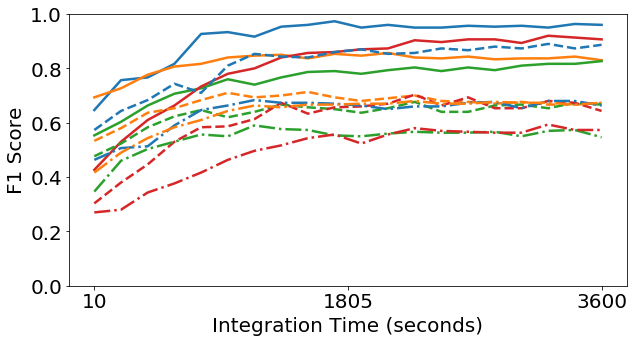
\includegraphics[width=\textwidth]{images/generalization-shielding-easy-05.png}
         \caption{}
         \label{fig:generalization-shielding-easy-05}
     \end{subfigure}

     \begin{subfigure}[b]{0.49\textwidth}
         \centering
         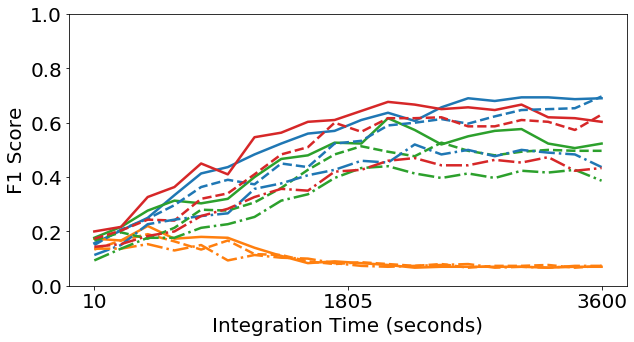
\includegraphics[width=\textwidth]{images/generalization-shielding-full-01.png}
         \caption{}
         \label{fig:generalization-shielding-full-01}
     \end{subfigure}
     \hfill
     \begin{subfigure}[b]{0.49\textwidth}
         \centering
         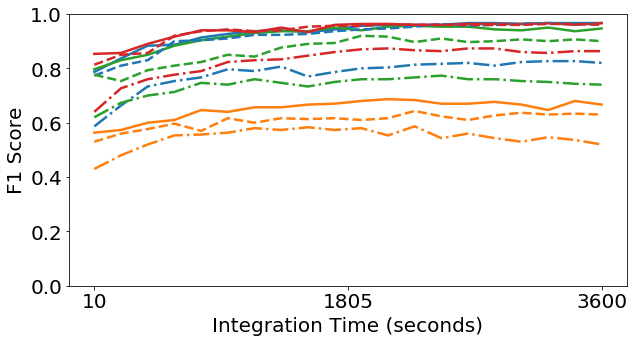
\includegraphics[width=\textwidth]{images/generalization-shielding-full-05.png}
         \caption{}
         \label{fig:generalization-shielding-full-05}
     \end{subfigure}
    \begin{tabular}{r@{: }l r@{: }l r@{: }l r@{: }l}
    DNN & Green & CNN & Red & DAE & Yellow & CAE & Blue\\
    \end{tabular}
    \begin{tabular}{r@{: }l r@{: }l r@{: }l}
    60\% & \blackline & 40\% & \blackdotline & 80\% & \blackdashdotline
    \end{tabular}
        \caption{Shielding generalization performance of the DNN, CNN with and without autoencoder pretraining. F1 score shown in averaged over five networks trained with data augmentation, Figures in the top and bottom row are trained using the simple and complete dataset and Figures in the first and second column are use spectra with signal-to-noise ratios of 0.1 and 0.5, respectively.}
        \label{fig:generalization_shielding_fixeddataset}
\end{figure}




\begin{figure}[H]
     \centering
     \begin{subfigure}[b]{0.49\textwidth}
         \centering
         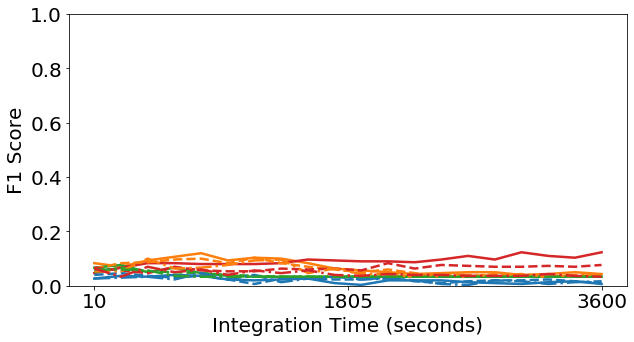
\includegraphics[width=\textwidth]{images/generalization-shielding-aug-easy-01.png}
         \caption{}
         \label{fig:generalization-shielding-aug-easy-01}
     \end{subfigure}
     \hfill
     \begin{subfigure}[b]{0.49\textwidth}
         \centering
         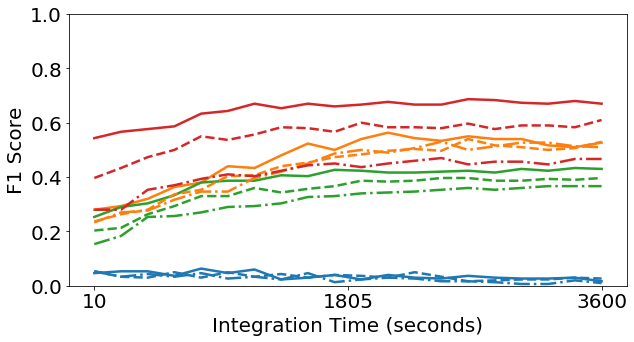
\includegraphics[width=\textwidth]{images/generalization-shielding-aug-easy-05.png}
         \caption{}
         \label{fig:generalization-shielding-aug-easy-05}
     \end{subfigure}

     \begin{subfigure}[b]{0.49\textwidth}
         \centering
         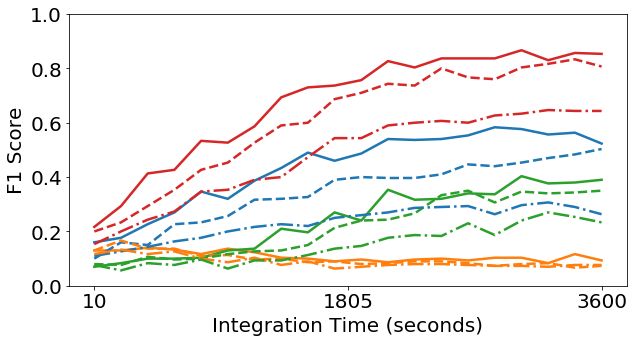
\includegraphics[width=\textwidth]{images/generalization-shielding-aug-full-01.png}
         \caption{}
         \label{fig:generalization-shielding-aug-full-01}
     \end{subfigure}
     \hfill
     \begin{subfigure}[b]{0.49\textwidth}
         \centering
         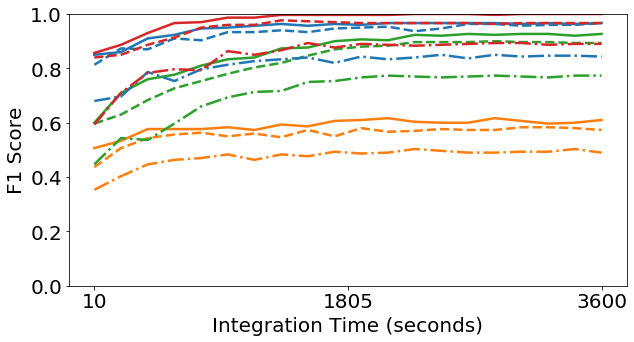
\includegraphics[width=\textwidth]{images/generalization-shielding-aug-full-05.png}
         \caption{}
         \label{fig:generalization-shielding-aug-full-05}
     \end{subfigure}
    \begin{tabular}{r@{: }l r@{: }l r@{: }l r@{: }l}
    DNN & Green & CNN & Red & DAE & Yellow & CAE & Blue\\
    \end{tabular}
    \begin{tabular}{r@{: }l r@{: }l r@{: }l}
    60\% & \blackline & 40\% & \blackdotline & 80\% & \blackdashdotline
    \end{tabular}
        \caption{Shielding generalization performance of the DNN, CNN with and without autoencoder pretraining. F1 score shown in averaged over five networks trained with data augmentation, Figures in the top and bottom row are trained using the simple and complete dataset and Figures in the first and second column are use spectra with signal-to-noise ratios of 0.1 and 0.5, respectively.}
        \label{fig:generalization_shielding_augdataset}
\end{figure}



\subsection{Generalization Dependence on Calibration.}

Datasets were simulated with various gain and offset setting.


\begin{figure}[H]
     \centering
     \begin{subfigure}[b]{0.49\textwidth}
         \centering
         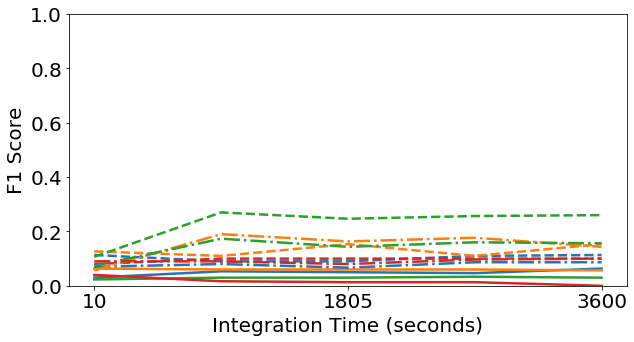
\includegraphics[width=\textwidth]{images/generalization-cal-easy-01.png}
         \caption{}
         \label{fig:generalization-cal-easy-01}
     \end{subfigure}
     \hfill
     \begin{subfigure}[b]{0.49\textwidth}
         \centering
         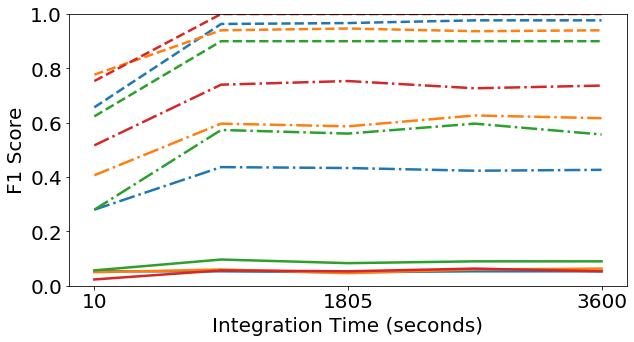
\includegraphics[width=\textwidth]{images/generalization-cal-easy-05.png}
         \caption{}
         \label{fig:generalization-cal-easy-05}
     \end{subfigure}

     \begin{subfigure}[b]{0.49\textwidth}
         \centering
         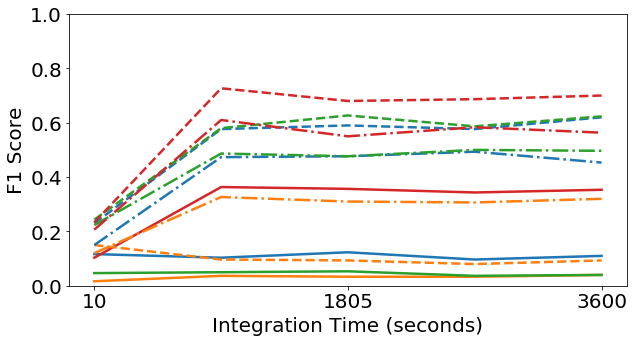
\includegraphics[width=\textwidth]{images/generalization-cal-full-01.png}
         \caption{}
         \label{fig:generalization-cal-full-01}
     \end{subfigure}
     \hfill
     \begin{subfigure}[b]{0.49\textwidth}
         \centering
         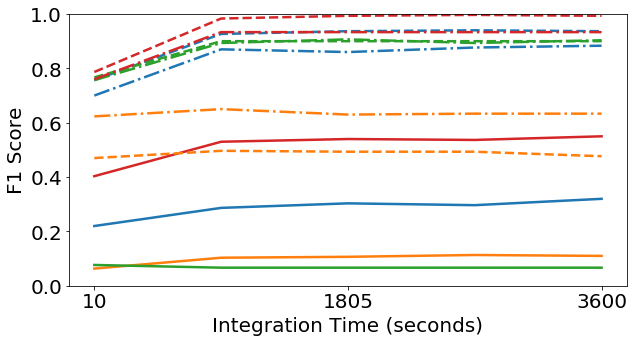
\includegraphics[width=\textwidth]{images/generalization-cal-full-05.png}
         \caption{}
         \label{fig:generalization-cal-full-05}
     \end{subfigure}
    \begin{tabular}{r@{: }l r@{: }l r@{: }l r@{: }l}
    DNN & Green & CNN & Red & DAE & Yellow & CAE & Blue\\
    \end{tabular}
    \begin{tabular}{r@{: }l r@{: }l r@{: }l}
    0.8 & \blackline & 1.0 & \blackdotline & 1.2 & \blackdashdotline
    \end{tabular}
        \caption{Calibration gain generalization performance of the DNN, CNN with and without autoencoder pretraining. F1 score shown in averaged over five networks trained with 10000 total dataset examples, Figures in the top and bottom row are trained using the simple and complete dataset and Figures in the first and second column are use spectra with signal-to-noise ratios of 0.1 and 0.5, respectively.}
        \label{fig:generalization_cal_fixeddataset}
\end{figure}




\begin{figure}[H]
     \centering
     \begin{subfigure}[b]{0.49\textwidth}
         \centering
         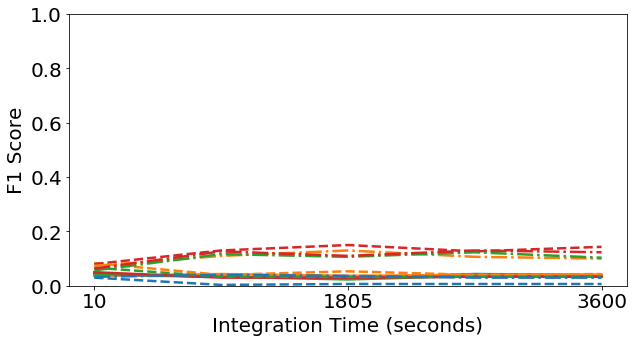
\includegraphics[width=\textwidth]{images/generalization-cal-aug-easy-01.png}
         \caption{}
         \label{fig:generalization-cal-aug-easy-01}
     \end{subfigure}
     \hfill
     \begin{subfigure}[b]{0.49\textwidth}
         \centering
         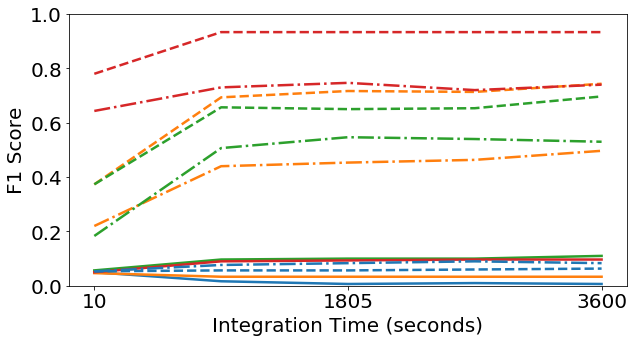
\includegraphics[width=\textwidth]{images/generalization-cal-aug-easy-05.png}
         \caption{}
         \label{fig:generalization-cal-aug-easy-05}
     \end{subfigure}

     \begin{subfigure}[b]{0.49\textwidth}
         \centering
         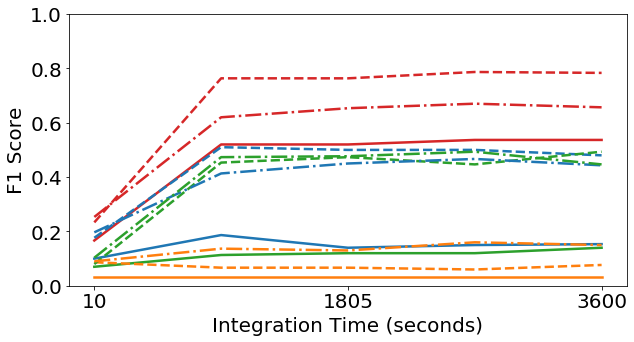
\includegraphics[width=\textwidth]{images/generalization-cal-aug-full-01.png}
         \caption{}
         \label{fig:generalization-cal-aug-full-01}
     \end{subfigure}
     \hfill
     \begin{subfigure}[b]{0.49\textwidth}
         \centering
         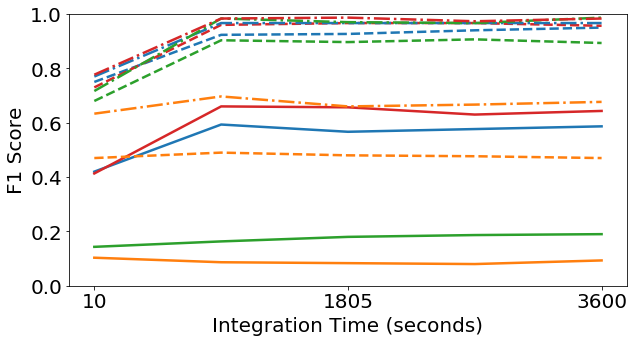
\includegraphics[width=\textwidth]{images/generalization-cal-aug-full-05.png}
         \caption{}
         \label{fig:generalization-cal-aug-full-05}
     \end{subfigure}
    \begin{tabular}{r@{: }l r@{: }l r@{: }l r@{: }l}
    DNN & Green & CNN & Red & DAE & Yellow & CAE & Blue\\
    \end{tabular}
    \begin{tabular}{r@{: }l r@{: }l r@{: }l}
    0.8 & \blackline & 1.0 & \blackdotline & 1.2 & \blackdashdotline
    \end{tabular}
        \caption{Calibration gain generalization performance of the DNN, CNN with and without autoencoder pretraining. F1 score shown in averaged over five networks trained with data augmentation, Figures in the top and bottom row are trained using the simple and complete dataset and Figures in the first and second column are use spectra with signal-to-noise ratios of 0.1 and 0.5, respectively.}
        \label{fig:generalization_cal_augdataset}
\end{figure}

% \subsection{Generalization Dependence on Changing Background.}

% Datasets were simulated with backgrounds different from the training set and real measured background. It is expected that the complete dataset will mistake background for isotopes more often than the simplified dataset because photopeaks are decreased by shielding.


\subsection{Results on Spectra for ANSI compliance}

This section shows model asymptotic performance vs integration time for ANSI compliance. Using N models (justified previously as asymptotic). 



\begin{table}[H]
\centering
\caption{Isotope combinations required for the ANSI standard \cite{ANSI}.}
\begin{tabular}{c}
Isotope Combinations \\ \hline
$^{137}$Cs + depleted uranium (DU) \\ % \hline
$^{99m}$Tc + HEU \\ % \hline
$^{201}$Tl + HEU \\ % \hline
$^{67}$Ga + HEU \\ % \hline
$^{131}$I + WGPu \\ % \hline
NORM + HEU \\ % \hline
NORM + WGPu \\ % \hline
\end{tabular}
\end{table}



\begin{figure}[H]
     \centering
     \begin{subfigure}[b]{0.9\textwidth}
         \centering
         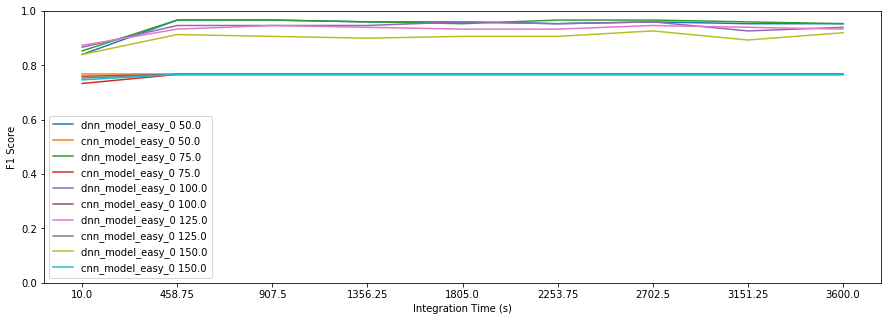
\includegraphics[width=\textwidth]{images/results_easy_distance_comparison}
         \caption{Simplified Dataset.}
         \label{fig:results_full_background_inject_simple}
     \end{subfigure}

     \begin{subfigure}[b]{0.9\textwidth}
         \centering
         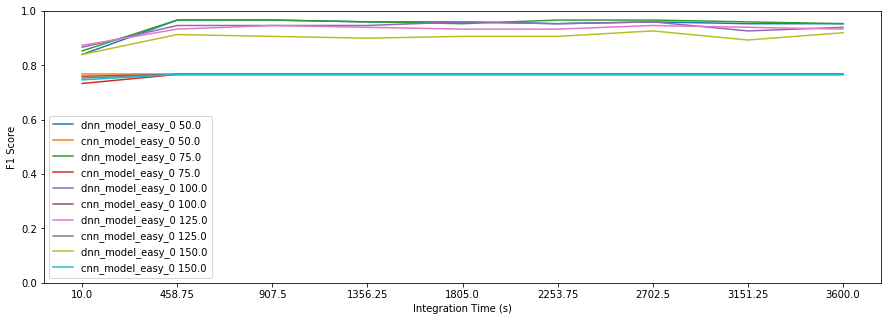
\includegraphics[width=\textwidth]{images/results_easy_distance_comparison}
         \caption{Complete Dataset.}
         \label{fig:results_full_background_inject_full}
     \end{subfigure}

        \caption{F1 score for models tested on ANSI isotope combinations.}
        \label{fig:results_full_background_inject}
\end{figure}



\subsection{Results on Measured Spectra}

This section shows model asymptotic performance vs integration time for a few different settings (different voltages, shielding)

To investigate how each model identified real spectra behind shielding and spectra with different calibrations, real spectra were measured. Sources include $^{137}$Cs, $^{60}$Co, $^{133}$Ba, and $^{152}$Eu. 


\subsubsection{Asymptotic Model Performance on Changing Voltage}

To see the generalization performance of the model to changing calibration, spectra with different voltages are recorded and their asymptotic performance compared.

Spectra were measured with different detector calibrations. A 2x2 Ortec NaI detector was set to 770 V, setting it's 1024th channel to 3 MeV. To capture a large range of calibrations, voltages varied from 720 V to 820 V in steps of 15 V. The $^{137}$Cs, $^{60}$Co, and $^{133}$Ba source had an activity of 1$\mu$C. For these sources, a source-to-detector distance of 14.25 mm was used to keep the cps on the detector from the source equal to the cps on the detector from background.

Figures \ref{fig:model_asymptotic_performance_co60} and \ref{fig:model_asymptotic_performance_cs137} show performance for isotopes with comparatively simplified spectra.


\begin{figure}[H]
     \centering
     \begin{subfigure}[b]{0.9\textwidth}
         \centering
         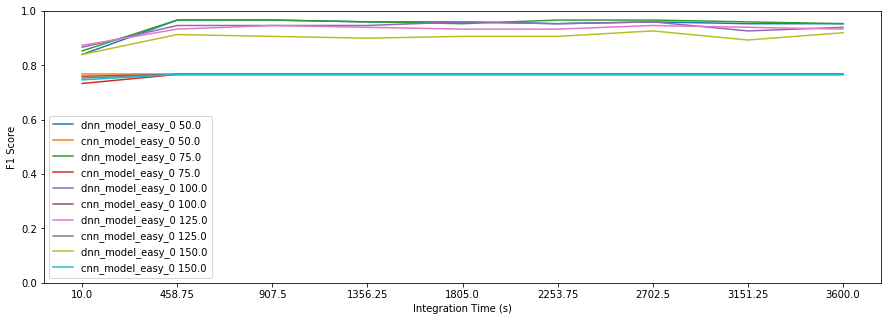
\includegraphics[width=\textwidth]{images/results_easy_distance_comparison}
         \caption{$^{60}$Co}
         \label{fig:model_asymptotic_performance_co60}
     \end{subfigure}

     \begin{subfigure}[b]{0.9\textwidth}
         \centering
         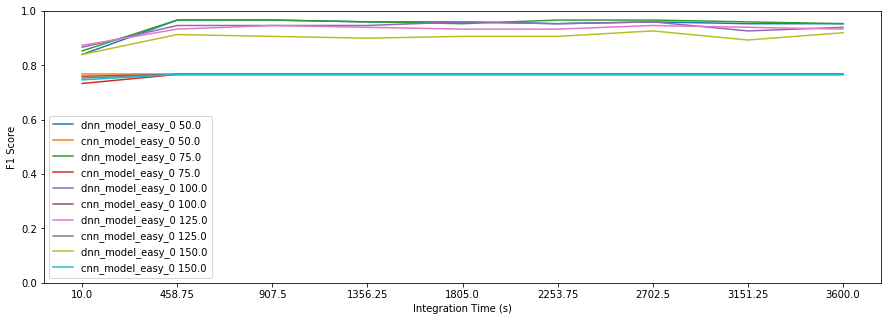
\includegraphics[width=\textwidth]{images/results_easy_distance_comparison}
         \caption{$^{137}$Cs.}
         \label{fig:results_easy_distance_comparison_full}
     \end{subfigure}
     
     \begin{subfigure}[b]{0.9\textwidth}
         \centering
         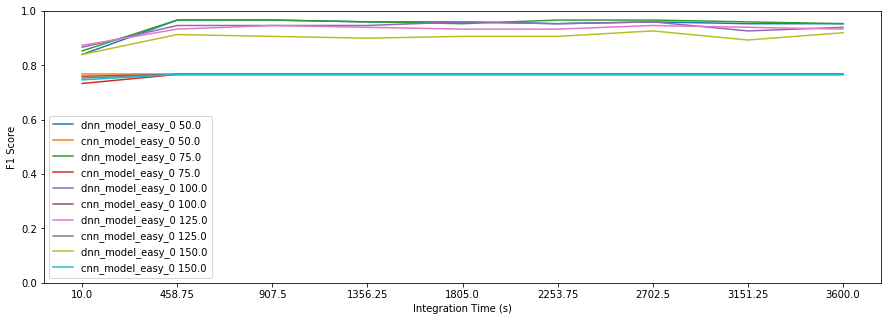
\includegraphics[width=\textwidth]{images/results_easy_distance_comparison}
         \caption{$^{152}$Eu.}
         \label{fig:results_easy_distance_comparison_full}
     \end{subfigure}
     
     \begin{subfigure}[b]{0.9\textwidth}
         \centering
         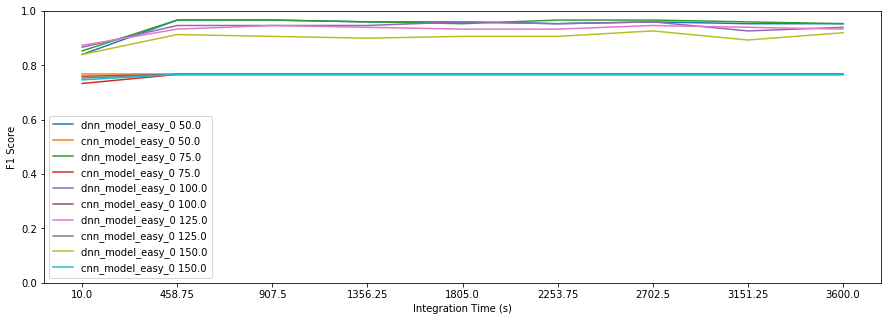
\includegraphics[width=\textwidth]{images/results_easy_distance_comparison}
         \caption{$^{133}$Ba.}
         \label{fig:results_easy_distance_comparison_full}
     \end{subfigure}

        \caption{F1 score for all models trained on the simplified dataset. Spectra measured with different gain settings.}
        \label{fig:results_easy_distance_comparison}
\end{figure}


\begin{figure}[H]
     \centering
     \begin{subfigure}[b]{0.9\textwidth}
         \centering
         \includegraphics[width=\textwidth]{images/results_easy_distance_comparison}
         \caption{$^{60}$Co}
         \label{fig:model_asymptotic_performance_co60}
     \end{subfigure}

     \begin{subfigure}[b]{0.9\textwidth}
         \centering
         \includegraphics[width=\textwidth]{images/results_easy_distance_comparison}
         \caption{$^{137}$Cs.}
         \label{fig:results_easy_distance_comparison_full}
     \end{subfigure}
     
     \begin{subfigure}[b]{0.9\textwidth}
         \centering
         \includegraphics[width=\textwidth]{images/results_easy_distance_comparison}
         \caption{$^{152}$Eu.}
         \label{fig:results_easy_distance_comparison_full}
     \end{subfigure}
     
     \begin{subfigure}[b]{0.9\textwidth}
         \centering
         \includegraphics[width=\textwidth]{images/results_easy_distance_comparison}
         \caption{$^{133}$Ba.}
         \label{fig:results_easy_distance_comparison_full}
     \end{subfigure}

        \caption{F1 score for all models trained on the complete dataset. Spectra measured with different gain settings.}
        \label{fig:results_easy_distance_comparison}
\end{figure}


\section{Chapter Conclusions}

The generalization performance results show that CNN's generally outperform other models and that autoencoder pretraining does not help with performance. Occasionally, at very low signal-to-background ratios, the DNN outperforms the CNN. To take advantage of this, it may be best to include a committee of CNN's and DNN's, or to train networks for specific ranges of integration time.

From the results shown in this chapter, using datasets of fixed sizes should be preferred over using online data augmentation. Online data augmentation usually reduced performance in each network


